%!TEX root = uiuc_2018_invitational.tex
\begin{problem}{Enclose These Cows}
{stdin}{stdout}
{1 second}{}{}

Farmer John has a herd of cows, and he plans to build a fence to enclose them so that no cow can escape (a cow on the boarder of the fence is not considered enclosed in the fence). There are already some poles on the field, and Farmer John can only build fence segments between these poles. Help Farmer John minimize the cost by computing the minimal length of a valid fence. \\
A figure representation of example 1 is drawn below. Black points stand for poles and white points stand for cows. Orange segments are the optimal fence. 
\begin{figure}[!h]
	\centering
	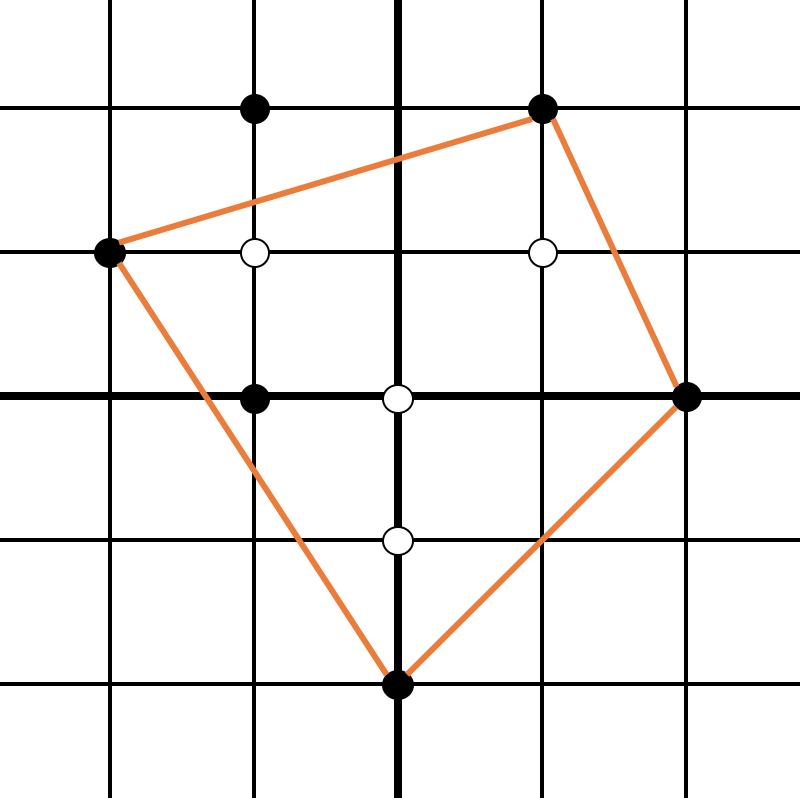
\includegraphics[scale=0.4]{sample1.png}
\end{figure}

\InputFile

The first line of input contains two integers $N, M$ ($1 \le N, M \le 100$). $N$ is the number of poles and $M$ is the number of cows. \\
In the following $N$ lines, each line contains two integers $x, y$ ($-10^6 \le x, y \le 10^6$), indicating that the coordinate of a pole is $(x, y)$ in 2-D Cartesian coordinate system. \\
In the following $M$ lines, each line contains two integers $x, y$ ($-10^6 \le x, y \le 10^6$), indicating that the coordinate of a cow is $(x, y)$ in 2-D Cartesian coordinate system. \\
All positions are guaranteed to be distinct. (i.e. no two poles, or two cows, or one pole and one cow, can take the same position)

\OutputFile

Print a line containing one real number, the minimal length of fence, \textbf{rounded to 2 digits after decimal point}. If it's impossible to build such a fence, output -1. 

\Examples

\begin{example}
\exmp{
6 4
2 0
1 2
-1 2
-2 1
-1 0
0 -2
0 0
1 1
-1 1
0 -1
}{%
11.83
}%
\exmp{
3 1
0 0
1 1 
-1 1
0 1
}{%
-1
}%
\end{example}

\end{problem}
